\subsubsection{(Some kind of) Case Based Reasoning}
To distinguish this application from the many existing solutions, some extra spice has been added in form of giving the user the option to let the application guess where he/she is going. To do this, a simplified version of case-based reasoning \cite{aam}, utilising is implemented, by logging each query made as a case. These data are stored locally in a database. In this database, the departing area, time of day, day of week and destination is stored for each query. Departing areas are squares of 500 $\times$ 500 meters, which has area codes stored in a separate table. Whenever a new log item is created, a new area is created if the origin location is not covered by an existing area . \\\\
\begin{figure}
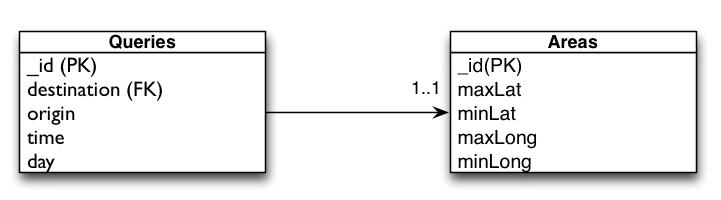
\includegraphics[scale=0.5]{Intelligence/database.png}
\caption{The database}
\end{figure}

To retrieve relevant cases, queries with similar origin and time are fetched from the database. Similarity means identical areas and somewhat similar time of day, for now +/- 2 hours is used. Then these cases are rated by the euclidean distance between case's and current time and weekday. The best matching destination is then presented to the user.
